\documentclass[12pt]{article}

\usepackage{fullpage}
\usepackage{graphicx, rotating, booktabs} 
\usepackage{times} 
\usepackage{natbib} 
\usepackage{indentfirst} 
\usepackage{setspace}
\usepackage{grffile} 
\usepackage{hyperref}
\usepackage{adjustbox}
\usepackage{amsmath}
\usepackage{siunitx}
\usepackage{multirow}
\setcitestyle{aysep{}}


\singlespace
\title{\textbf{The Sources of Alliance Treaty Depth}}
\author{Joshua Alley\footnote{Graduate Student,
Department of Political Science, Texas A\&M University.}}
\date{\today}

\bibliographystyle{apsr}

\begin{document}

\maketitle 

\doublespace 

\begin{abstract}
Why do states make formal commitments of defense coordination and cooperation in military alliance treaties? 
I argue that states use treaty depth to increase the credibility of their alliance commitments while managing entrapment risk. 
Democracies are especially inclined to form deep alliances because depth increases reliability without exposing leaders to domestic audience costs or entrapment.
Unlike unconditional military support, depth limits audience costs, so I expect that democratic alliance leadership increases treaty depth but decreases the likelihood of unconditional military support. 
I test this claim with an analysis of offensive and defensive alliances from 1816 to 2007 and a short case study of the North Atlantic Treaty Organization.
I find that more democratic institutions in the most capable alliance member increase treaty depth, but do not affect unconditional military support.   
The argument and findings challenge claims that democracies prefer limited alliance commitments. 
\end{abstract}


\newpage 


\section{Introduction}


% Start with hook: maybe a story of a deep and shallow alliance 
Why do states make deep alliance treaties? 
Some alliances supplement military support promises with commitments of peacetime defense cooperation and policy coordination. 
Deep alliances include promises like basing rights, international organizations, policy coordination, and integrated military command.
I argue that states use treaty depth to increase the credibility of their alliance commitments while managing the risk of entrapment, so states with high audience costs from abandoning an ally are more likely to use depth to reassure. 

 
The sources of treaty depth are worth studying because states frequently employ this source of credibility.
Half of all ATOP alliances with offensive or defense obligations have some treaty depth.
Moreover, treaty depth changes alliance politics. 
Credibility from deep alliances encourages non-major power members to reduce military spending.  
Thus, treaty depth affects alliance politics by shaping treaty credibility and the distribution of military spending among members. 


% Describe question and contribution of the paper
Despite the prevalence and consequences of alliance treaty depth, we have little idea when states add depth to their alliances.\footnote{\citet{Mattes2012} examines the causes of military institutionalization.}
In this paper, I explain when states make deep alliance treaties.
I start with the premise that depth is one of two ways that states can increase the credibility of their alliance commitments, and argue that domestic political institutions shape whether states prefer treaty depth.
Treaty depth and unconditional military support are two costly ways states can increase the credibility of their alliance commitments.
Because democratic leaders are concerned with the audience costs of treaty violation, they prefer to reassure allies with deep alliance treaties.
Depth increases alliance credibility with less exposure to domestic audience costs. 
On the other hand, unconditional military support exposes leaders to entrapment or the audience costs of treaty violation, so democracies often make conditional alliance commitments \citep{Mattes2012, Chibaetal2015}.
Therefore, I expect that democracies will often form deep alliances with conditional promises of military support. 


I test the argument with a statistical analysis of offensive and defensive alliances from 1816 to 2007 and an illustrative case study of the North Atlantic Treaty Organization (NATO).
I estimate a series of statistical models, including bivariate models that adjust for unobserved correlations between treaty depth and unconditional military support \citep{Braumoelleretal2018}. 
The case study shows that democratic alliance leaders fear entrapment, but are willing to use treaty depth to reassure allies \citep{SeawrightGerring2008, Seawright2016}. 
I find consistent evidence that alliances with democratic leaders have higher treaty depth.
Evidence that democratic alliance leadership decreases the probability of unconditional military support is less consistent, however. 


% Para on implications: sources of credibility and reassurance are connected
This paper contributes to three strands of scholarly inquiry.
First, it adds to a growing literature on alliance treaty design.  
Existing scholarship examines parts of treaty design in isolation \citep{Benson2012, Mattes2012, Chibaetal2015}, but I show how different sources of credibility in alliance treaty design are connected. 
My argument considers how audience costs shape preferences for different types of reassurance, and some empirical models account for the relationship between different sources of alliance credibility. 


% Paragraph on the importance of democracy in alliance pol
Second, this paper contributes our understanding of how domestic politics affect international alliances. 
Scholars have long acknowledged that democracy and alliances are connected \citep{LaiReiter2000, GiblerWolford2006, Mattes2012, Warren2016, McManusYarhi-Milo2017}. 
Existing scholarship suggests that democracies prefer limited commitments \citep{Mattes2012, Chibaetal2015, FjelstulReiter2019} because they are more likely to make conditional promises of military support. 
\citet{Chibaetal2015} write that ``domestic costs can make democratic states wary of engaging in agreements requiring broad and/or deep cooperation.'' 
My argument suggests that even if democracies screen the scope of their commitments carefully, they form deeper alliances on other dimensions.  
As a result, the net effect of the connection between democracy, alliance design and treaty credibility requires further research.
Scholars often claim that audience costs make democratic commitments more credible \citep{Gaubatz1996, Leedsetal2009, PotterBaum2014, DigiuseppePoast2016}, but this relationship is disputed \citep{GartzkeGleditsch2004, DownesSechser2012}.  
Third, the argument is part of a rich literature on domestic politics and international cooperation, e.g. \citep{DownesRocke1995, Fearon1998, Leeds1999, MattesRodriguez2014}. 
If democracies reassure partners with deep alliance commitments, audience costs sometimes push democracies to undertake international commitments with less electoral salience. 


% This paper is needed: don't know much about depth
This paper fills an important gap in the literature. 
The process of alliance treaty negotiation and design is understudied \citep{Poast2019a}, and there is even less research on treaty depth. 
In the nascent alliance treaty design literature, most scholarship examines conditions on military support.
\citet{Benson2012} shows that foreign policy disagreements and revisionist protege states increase the likelihood of limited military support and \citet{Kim2011} claims that states use conditional obligations to escape entrapment. 
\citet{Mattes2012} finds that joint democracy increases the probability of conditional alliance obligations, as well as little evidence that alliance symmetry and history of violation affect conditionality. 
\citet{Chibaetal2015} add to to existing work on limited obligations with evidence that democracies are more likely to form alliances with conditional military support or consultation. 
Last, \citet{FjelstulReiter2019} argue that democracies prefer incomplete alliance contracts as another means of limiting audience costs. 


Two other studies of alliance treaty design examine concepts that are similar to treaty depth, but both treat depth and conditions on military support as independent sources of credibility.   
First, \citet{Mattes2012} argues that members of symmetric bilateral alliances where one partner has history of violation will be more likely to use conditions on military support, issue linkages, and military institutionalization to increase treaty reliability. 
Her measure of military institutionalization \citep{LeedsAnac2005} is close to my conceptualization of treaty depth, and Mattes finds that symmetric alliances where one partner has a history of violation have higher institutionalization.
\citet{Mattes2012} makes an important contribution, but does not differentiate between the costs and benefits of different sources of alliance credibility, and her military institutionalization measure understates the extent of variation in treaty depth.  
Second, \citet{BensonClinton2016} find that foreign policy agreement, major power involvement and treaty scope are all positively correlated with depth, while checking the validity of a latent measure of how costly alliance obligations are in general. 
Benson and Clinton's latent measure of depth includes secrecy and issue linkages, so it captures a broader concept than deep military cooperation. 
Neither study provides an explanation for why states might prefer depth to other sources of alliance credibility. 


Therefore, we still do not understand why states add treaty depth to alliances, especially in relation to other sources of alliance credibility. 
To explain this, I compare treaty depth to unconditional military support.  
Both treaty depth and unconditional military support increase alliance credibility, but they have different costs.
Relative concern with these costs especially entrapment and audience costs, depends on domestic political institutions. 


% roadmap for the paper 
The paper proceeds as follows. 
In the next section, I lay out the argument and hypothesis. 
Then I describe the data and research design. 
The final sections discuss the results and implications. 


\section{Argument}


In this argument, I first establish a definition of treaty depth.  
After that, I offer a general explanation of the costs and benefits of treaty depth, relative to unconditional military support. 
Based on the general framework, I then detail why democracies often increase treaty depth, but are less likely to offer unconditional military support. 


% define alliance treaty depth
Alliance depth is the extent of defense cooperation a treaty formalizes. 
Deep alliances require additional military policy coordination and cooperation. 
While shallow alliances stipulate more arms-length ties between members, deep treaties lead to closer cooperation through intermediate commitments that fall between treaty formation and military intervention. 
Defense cooperation in a deep alliance takes many forms. 
Allies can promise an integrated military command, military aid, a common defense policy, basing rights, international organizations, specific capability contributions or companion military agreements. 


Treaty depth helps states address opportunism in commitments of military support.
Alliances are self-enforcing contracts or institutions \citep{Leedsetal2002, Morrow2000}.
When faced with external threats in an anarchic international system, states form alliances to aggregate military capability and secure their foreign policy interests \citep{Altfield1984, Smith1995, Snyder1997, FordhamPoast2014}. 
Treaties that formalize promises of military support take many forms \citep{Leedsetal2000, Leedsetal2002, Benson2012, BensonClinton2016}. 
Treaty design shapes the costs and benefits of treaty participation and addresses potential opportunistic behavior. 
Beyond the benefit of potential military support, alliances also clarify international alignments \citep{Snyder1990} and support economic ties \citep{Gowa1995, Li2003, Long2003, Fordham2010, WolfordKim2017}. 
The costs of alliances include lost foreign policy autonomy \citep{Altfield1984, Morrow2000, Johnson2015}, and the potential consequences of opportunistic behavior. 
Opportunism in alliances includes abandonment, or the failure of alliance members to honor their commitments \citep{Leeds2003a, BerkemeierFuhrmann2018}, entrapment in unwanted conflicts \citep{Snyder1984}, and free-riding \citep{Morrow2000}.   


% process of alliance negotiations: establishing a credible commitment. 
To form an alliance, states must have sufficient overlap in foreign policy interests \citep{Morrow1991, Smith1995, FordhamPoast2014}, especially their proposed war plans \citep{Poast2019a}. 
By making a formal alliance treaty, members attempt to increase the credibility of military interventions \citep{Morrow2000}. 
Alliance members and other states use the costs of the alliance commitment to assess treaty reliability. 
While alliance formation alone adds some credibility, treaty depth or unconditional promises of military support add further credibility. 
Depth and unconditional military support are both costly commitments that alliance members and other states can observe. 


% balance credible commitment and entrapment 
Efforts to ensure alliance credibility can increase the risk of entrapment in unwanted conflicts, however. 
If an ally invokes a treaty when a state would rather stay out, a dilemma follows--- a state can either fight in an unwanted war, or pay the reputational \citep{Gibler2008, Crescenzietal2012} and audience \citep{Fearon1997} costs of treaty violation.  
Whether an alliance imposes conditions on military support clearly shows the relationship between credibility and entrapment.
Conditional alliances limit promises of intervention to particular regions, conflicts, or instances of non-provocation \citep{Leedsetal2000}. 
When alliance members fear divergent allied interests will create an entrapment or violation dilemma, they constrain military support to specific circumstances \citep{Kim2011, Benson2012}.\footnote{Such deliberate design of alliances means clear instances of entrapment are rare \citep{Kim2011, Beckley2015}.} 
Conversely, offering unconditional military support indicates high shared foreign policy interests and less fear of entrapment.
Under unconditional commitments of intervention alliance members hazard entrapment or the costs of treaty violation in more circumstances. 
Therefore, unconditional alliances are a costly signal of substantial foreign policy agreement, which adds credibility.  


When states make unconditional promises of military support, alliance members have substantial foreign policy agreement.
Alliance members face a time-inconsistency problem, however \citep{LeedsSavun2007}. 
Although conditions on military support are fixed, foreign policy interests change. 
If interests change and a partner calls on a state to fight in an unwanted conflict, states must bear either entrapment or the audience costs of treaty violation.
When audience costs are less costly than fighting, states will often choose to violate the treaty and bear the audience costs.   
But states with high audience costs will be more sensitive to engagement in unwanted conflicts, because violation is more costly. 
Therefore, states with high audience costs will be less likely to offer unconditional military support  \citep{Chibaetal2015}. 


% Part 2: depth
Unconditional military support is not the only source of alliance credibility, however. 
Treaty depth is an alternative way to reassure allies that has less risk of entrapment. 
Depth shapes the perceived reliability of an alliance by providing opportunities for states to fulfill treaty obligations in peacetime \citep{Morrow1994}. 
When states implement deep obligations, it provides a sunk cost signal of commitment.
Observing that alliance members adhere to peacetime promises suggests that they will also honor promises of military support. 


How does depth limit the risk of entrapment?   
Failure to implement deep alliance provisions provides an observable signal of foreign policy divergence short of war.
Furthermore, policy coordination in a deep alliance gives states more influence over allied actions and policies. 
Bases, joint organization and policy coordination are all potential checks on entrapment.
Coordinating policies and plans over time allows states to ensure that their joint war plans still line up, and that neither member faces a prohibitive risk of abandonment or entrapment.  


% depth has a different cost: FP autonomy
Treaty depth mitigates the reliability and entrapment dilemma, but it has a different cost. 
Besides opportunism, lost foreign policy autonomy is the other major cost of alliance participation. 
Deep alliances reduce foreign policy autonomy more than other alliances.
Cooperating and coordinating policy with allies reduces the ability of states to make unilateral decisions. 
There are also practical hurdles to unwinding foreign bases, international institutions and integrated military commands. 


% summarize difference in costs
Though depth and unconditional military support both increase alliance credibility, they do so in different ways. 
Conditions on military support do not change without a treaty renegotiation, and the costs of fighting are hypothetical unless the alliance is invoked.  
Highly conditional alliances are less costly in expectation, which reduces their credibility but guards against entrapment. 
Conversely, the sunk costs of depth can be observed without invoking promises of military support and address time-inconsistency problems.
Depth and cooperation with allies increases credibility with less risk of entrapment, but leads to greater foreign entanglement.   


% Combine the two
Whether states are more concerned with entrapment or foreign entanglement therefore shapes how they reassure their alliances. 
When states fear entrapment and do not want to face the audience costs of treaty violation, they will form deep alliances with conditional promises of military support.\footnote{Prospective alliance members could also make an arms-length alliance commitment with neither depth nor unconditional military support, or use treaty depth to address time-inconsistency problems with unconditional military support.}
Therefore, states with high audience costs for violating promises of military support and relatively low concern with foreign entanglement in the leader's key foreign policy audiences will use treaty depth to increase the credibility of their alliances. 
Domestic political institutions shape leaders' foreign policy audiences and the balance of these concerns.  
Due to high audience costs of military support and low public concern with foreign entanglement short of military intervention, I expect that alliances with democratic leaders will be more likely to have limited military support and high depth. 



\subsection{Democratic Alliance Leadership and Treaty Design}


% Talk about voters
Democracies use treaty depth to reassure partners because depth increases the perceived reliability of their alliances while shielding them from domestic audience costs. 
Violating international promises can have audience costs for democratic leaders.
Democratic leaders fear that if they violate international commitments, public disapproval will lead to their removal from office.  
Audience costs apply more to unconditional military support than treaty depth, however. 
Two characteristics of the public audience in democracies encourage leaders to use treaty depth in alliance commitments.  
First, audience costs increase as crises escalate \citep{Tomz2007}, so promises of military support are salient to the democratic public.  
Second, the public in democracies lacks substantial foreign policy information, so foreign entanglements short of war from treaty depth have limited salience in domestic politics. 
Democratic voters are unlikely to have much information or strong preferences about defense cooperation with allies. 
Although foreign policy elites may dispute changes in commitment to a deep alliance, such dissent is unlikely to translate 
into meaningful public opposition and electoral concerns.


% How do allies respond?
Unlike in domestic politics, differences in treaty depth and the implementation of alliance promises are salient in international politics. 
Allied states and potential adversaries can gather useful information from treaty depth. 
By including peacetime costs in a deep treaty, alliance members signal alliance reliability. 
Implementing costly promises of military aid, bases, or policy coordination indicates commitment. 
This increases allied confidence that democracies will honor their treaty obligations. 
Therefore, democracies can use treaty depth to signal international commitment with less exposure to domestic audience costs. 


% analogous to optimal obfuscation in trade policy
The way democracies use treaty depth in alliances is analogous to their reliance on non-tariff barriers in trade policy.
\citet{Kono2006} argues that because non-tariff barriers are more complex, voters lack sufficient information about their impact on consumer prices.
Tariffs, on the other hand, translate directly into prices in ways that are easy to understand.
The complexity of non-tariff barriers makes them less vulnerable to electoral attack, so democracies engage in ``optimal obfuscation'' and substitute non-tariff barriers for tariffs. 
In the same way, unconditional promises of military support and treaty depth both affect international relations, but the former is salient for voters and the latter is not. 
Unconditional military support is easy to explain to voters, but treaty depth is not. 
Therefore, democratic leaders can use treaty depth to manage international relations with fewer domestic political consequences.


% What is it exactly about democracies
Open political competition for leadership, contested elections and legal constraints on executive action are three possible sources of audience costs in democracies. 
Open recruitment of leaders through elections increases the chance a leader is removed from office. 
Political competition allows opposition groups to hold leaders to account for foreign policy shortcomings. 
For leaders to fear replacement, there must be a viable opposition offering alternative policies \citep{PotterBaum2014}.
Democratic leaders also face legal constraints on their foreign policy, and violating these restraints could generate audience costs. 
I examine the relative weight of these three mechanisms in the empirical analysis.  


% What about different types of autocracies? 
This argument uses the limited domestic audience costs and reassurance benefits of treaty depth to explain why democracies often form deep alliances. 
What about autocracies? 
Some autocratic leaders, especially in single-party states, also face high audience costs for backing down in military conflicts due to scrutiny from domestic elites \citep{Weeks2014}.
Domestic elites in single party states are a different audience than the public in democracies, however.  
Party elites are more informed about foreign policy than the public in democracies, so they can also impose costs on leaders that violate promises of treaty depth. 
In general, no autocratic audience has the combination of limited foreign policy information and high audience costs of military intervention as democracies.
Single-party and military regime leaders face an informed domestic elite, and personalist leaders have few meaningful foreign policy audiences. 
Therefore, assuming that all autocracies are equivalent, relative to democracies is sufficient for this paper.\footnote{Examining heterogeneity among autocracies in alliance treaty design is an interesting subject for future research, however.} 


% Sources of democratic influence in alliance negotiations. 
Of course, democracies need not get all they want in alliance negotiations. 
Following \citep{Mattes2012}, I expect that more capable states have greater influence on alliance negotiations, because their partners lose out on more foreign policy benefits if they are out of the alliance.
The most capable state is often the alliance ''leader,'' which increases the weight of their preferences and concerns. 
Therefore, to understand how democracy shapes alliance treaty design, I conceptualize democratic influence in terms of the political regime type of the most capable alliance member. 


% express the key hypothesis
Due to the limited audience costs of treaty depth, democracies will often design deep alliance treaties to increase the credibility of their alliance commitments. 
As the democracy of the most capable alliance member at the time of treaty formation increases, treaty depth will increase. 


\begin{quote}
\textsc{Treaty Depth Hypothesis: As the average democracy of the most capable alliance member at the time of formation increases, alliance treaty depth will increase.}
\end{quote} 


% End with a well-established result: democracy and conditional obligations
I also expect that democratic alliance membership will reduce the probability of unconditional military support, because backing out of a promised military intervention generates substantial audience costs. 
This second claim matches existing arguments and findings. 
\citet{Mattes2012} and \citet{Chibaetal2015} both show that democracies are more likely to design conditional alliances. 
They attribute this finding to higher audience costs of violating international commitments in democracies. 
Because democratic leaders face substantial audience costs from violating their international commitments, leaders design more limited commitments that are easier to fulfill. 
On the other hand, autocracies may be more willing to promise unconditional military support, because backing out of unwanted conflicts has lower audience costs. 
Based on this logic, increasing the democracy of the most capable member when the alliance formed should reduce the probability of unconditional military support.


\begin{quote}
\textsc{Unconditional Military Support Hypothesis: As the average democracy of the most capable alliance member at the time of formation increases, the probability that the alliance offers unconditional military support will decrease.}
\end{quote} 


% Discuss the correlations
Depth and conditional obligations in democratic alliances are complementary, as depth substitutes for unconditional military support as a source of credibility. 
Limiting alliance commitments through conditional military support reduces audience costs because it is easier for democratic leaders to backtrack on military support. 
Leaders can claim that the conditions for intervention were not met, or that new information obviates the alliance commitment \citep{LevenduskyHorowitz2012}. 
Because allied states understand these limits, conditional alliances will increase reliability concerns. 
This may undermine the credibility of the alliance, as unreliable pacts invite challengers \citep{Smith1995}. 
But even if conditional military support reduces the credibility of democratic alliances, treaty depth strengthens the alliance. 
Thus, depth reassures the allies of democracies, who might otherwise have reliability concerns from conditional military support. 


% Taking the two hypotheses together
Scholars often use the finding in previous research that democracies prefer conditional alliances to claim that democracies make limited alliance commitments. 
But if democracies frequently add depth to their alliance treaties, democratic alliances are limited on one dimension and deep on another. 
Furthermore, deep alliances may produce closer security ties than unconditional military support.  


% can cut this if needed. 
There is an important caveat to this argument--- I am interested in institutional design, not implementation.
Alliance treaty depth is not always implemented fully, as treaty aspirations are not fully realized, or work poorly. 
To give one example, several deep Arab alliances never realized their full intention due to internal political divisions.  
For treaty depth to increase treaty credibility, states must implement some promises, however. 


I expect that more democratic alliance membership will increase treaty depth, but reduce the likelihood of unconditional military support.  
This occurs because democracies prefer to use treaty depth to reassure their partners. 
In the next section, I describe how I test this claim about the association between democratic alliance leadership and the two sources of alliance credibility. 



\section{Research Design}

 
I expect that democracy among alliance members will increase treaty depth and decrease the probability of unconditional military support. 
Furthermore, the processes behind conditions on military support and treaty depth may be related, as both are sources of credibility. 
I examine these claims with a series of statistical models and an illustrative case study of NATO. 
I first describe the key variables in the analysis, then provide more detail on the estimation strategy. 


% start with data
To examine my predictions that democracies tend to produce conditional alliances with substantial depth, I employ data from the Alliance Treaty Obligations and Provisions Dataset \citep{Leedsetal2002}. 
The sample includes 289 alliances with either offensive or defensive obligations, which is the set of treaties with military support.\footnote{Results are robust to adjusting for non-random selection into alliances. See the appendix for details.} 
I measured treaty depth using a semiparametric mixed factor analysis of eight ATOP variables \citep{Murrayetal2013}.\footnote{\textbf{\url{https://github.com/joshuaalley/arms-allies/blob/master/manuscript/arms-allies-paper.pdf}} contains more details on the measure.}
The depth measure is a weighted combination of ATOP's defense policy coordination, military aid, integrated military command, formal organization, companion military agreement, specific contribution, and bases variables. 
Each of these individual indicators increases alliance treaty depth, but defense policy coordination and an integrated command have the largest positive association, as shown in the top panel of \autoref{fig:loadings-measure}. 


\begin{figure}[hbtp]
\centering
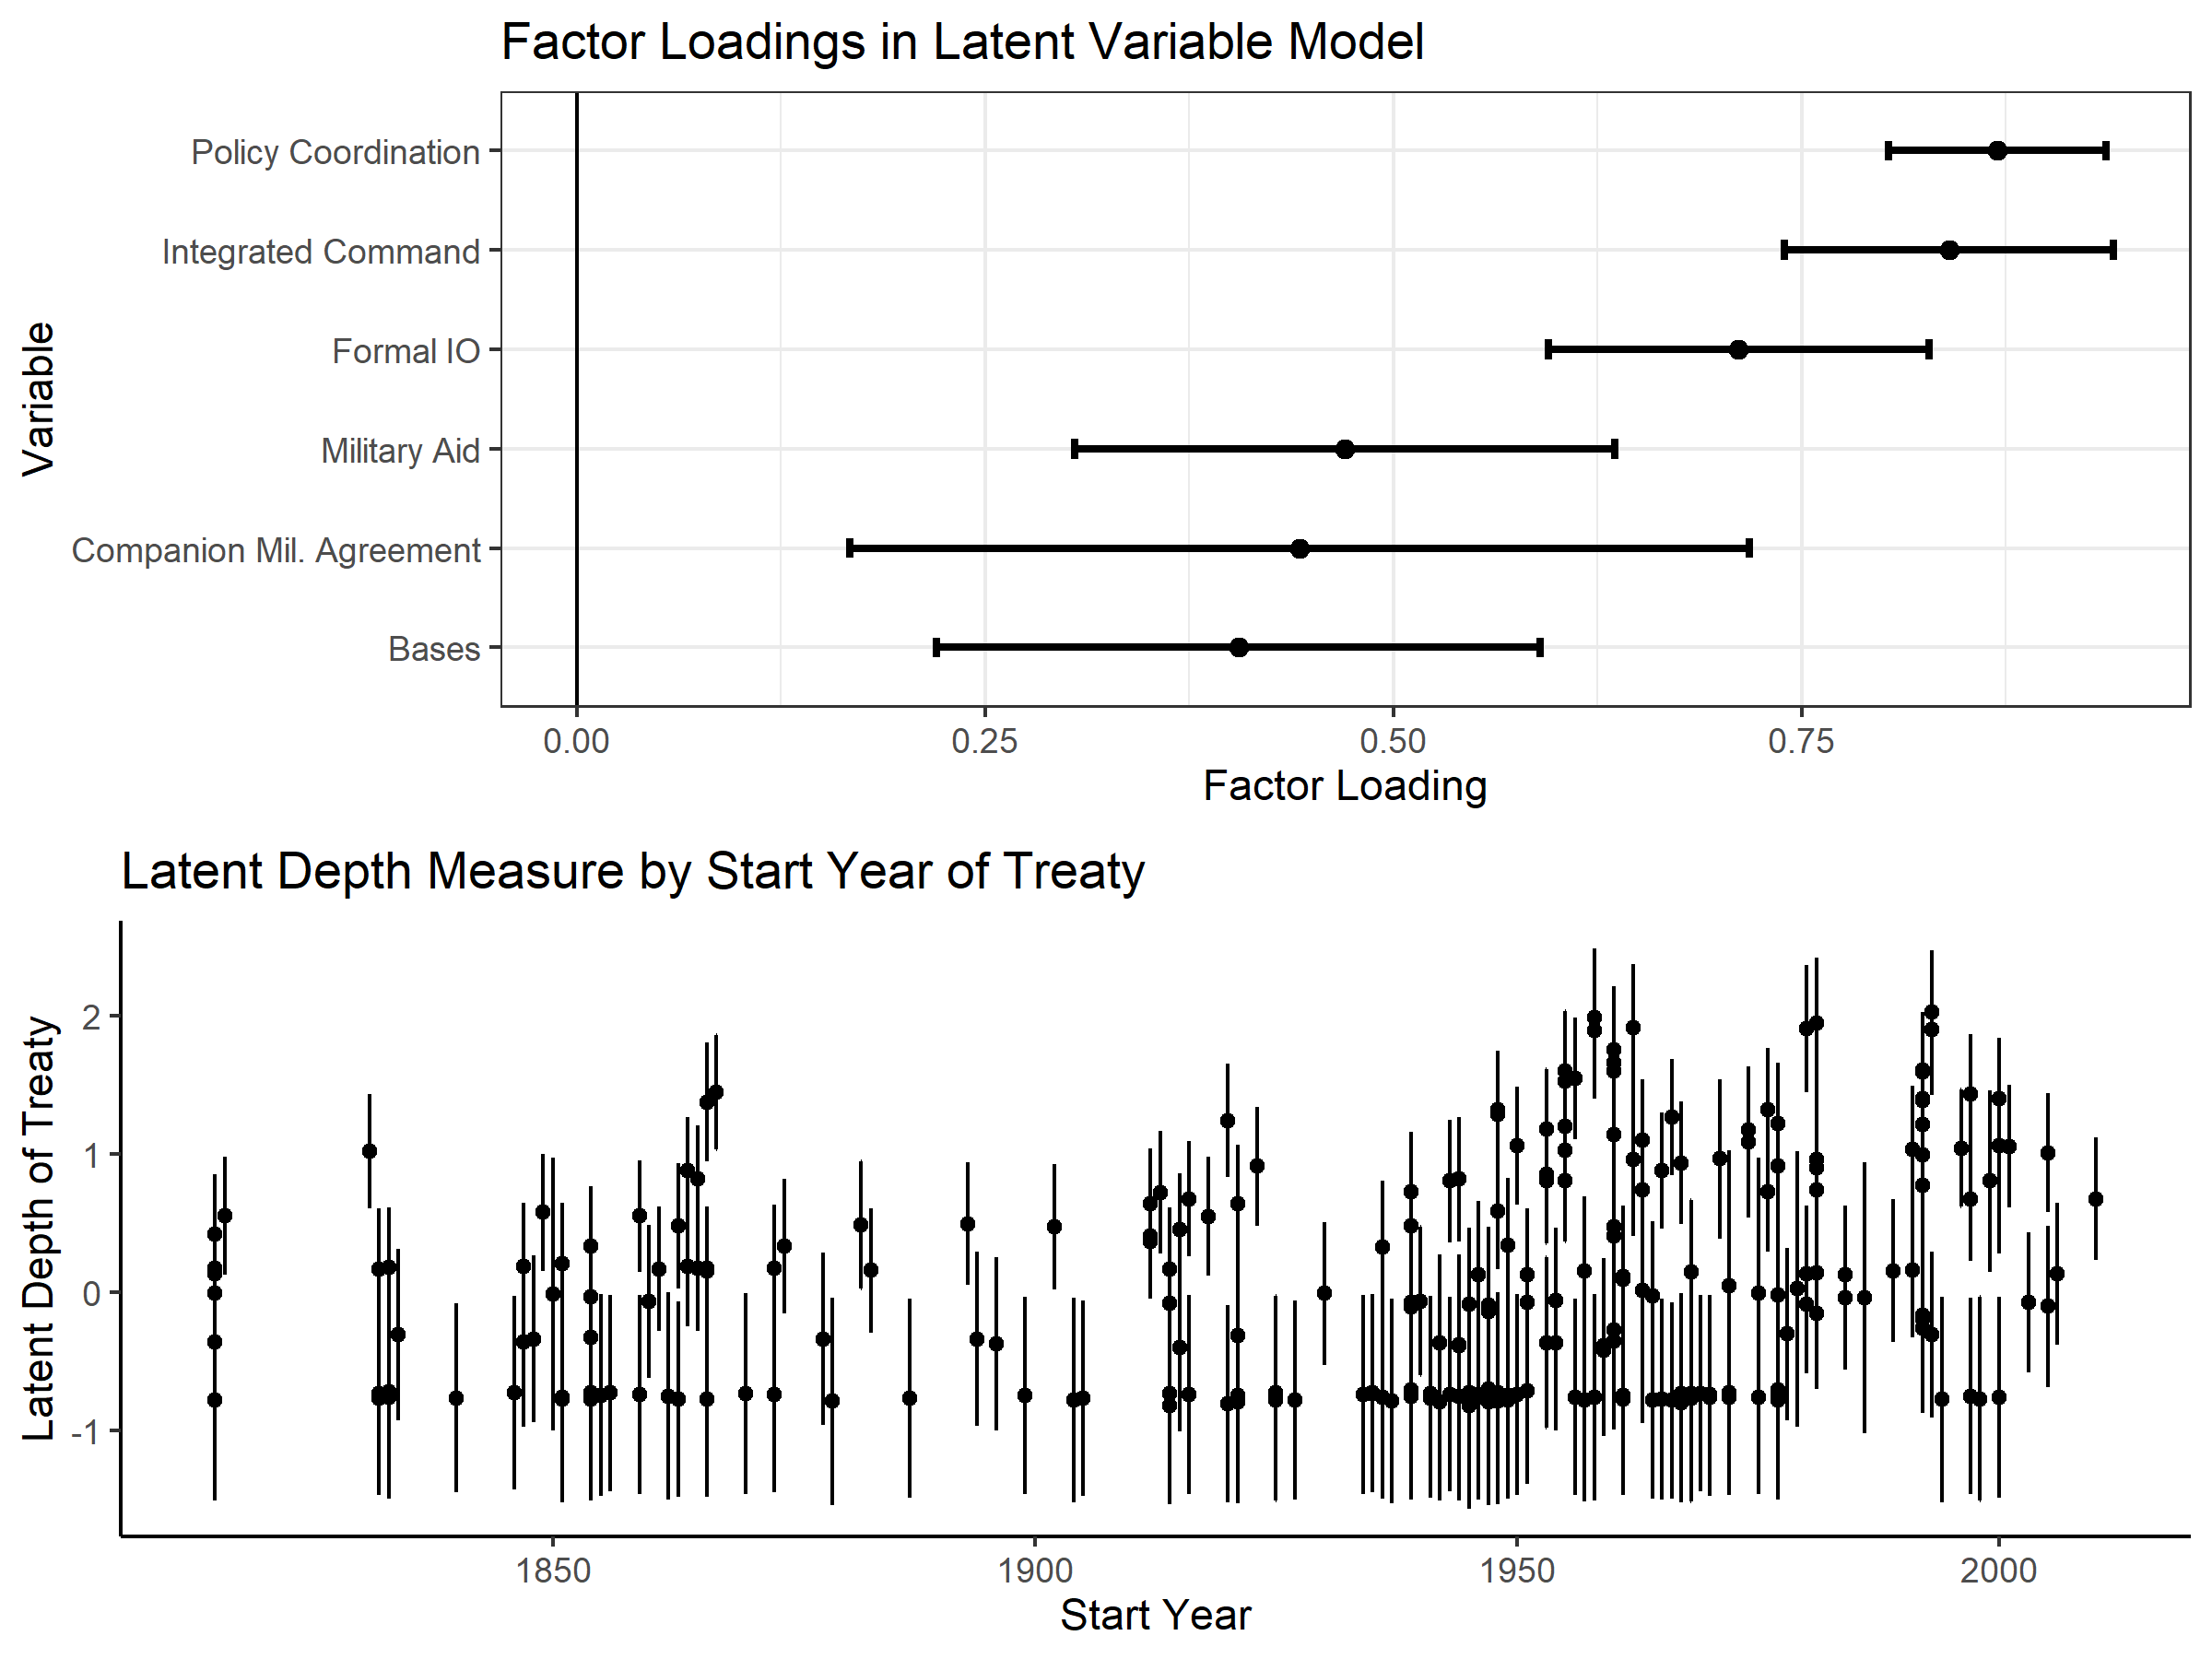
\includegraphics[width=0.95\textwidth]{../figures/loadings-measure.png}
\caption{Factor Loadings and posterior distributions of latent alliance treaty depth measure.}
\label{fig:loadings-measure}
\end{figure}


The measurement model predicts the likely value of treaty depth for each alliance using the factor loadings. 
The distribution of depth is summarized by the bottom panel of \autoref{fig:loadings-measure}. 
There is substantial variation in alliance treaty depth. 
Around half of all formal alliance treaties have some depth, and there is wide variation in how much depth is present.
I measure treaty depth using the posterior mean of the latent depth posterior for each alliance. 
This summarizes the central tendency of latent treaty depth, and results are robust to accounting for uncertainty in the latent measure. 


The other outcome variable is a dummy indicator of unconditional military support. 
Using ATOP's information on whether defensive or offensive promises are conditional on specific locations, adversaries, or non-provocation, I set this variable equal to one if the treaty placed no conditions on military support.
123 of 289 alliances in the data offer unconditional military support. 


The key independent variable is the democracy score of the most capable alliance members when the treaty formed. 
I use the POLITY measure of political institutions to measure democracy, and code the alliance leader as the state with the largest CINC score \citep{SingerCINC1988}.
This measure captures domestic institution and potential sensitivity of the leading state in the alliance to audience costs and entrapment.
It also emphasizes the influence of the most capable alliance member.\footnote{I find similar results with a model that uses the proportion of democracies as the key independent variable, which I report in the appendix. The proportion of democracies measures the prevalence of democratic membership, and it has a strong positive correlation with the democracy of the most capable member.}    


% Justify this approach
A common alternative measure of allied democracy is a dummy variable which is equal to one if all alliance members have a polity score greater than five.\footnote{Only 25 of the 285 alliances in my data clear this joint democracy threshold.}
I prefer the leading alliance member democracy score to this dummy for two reasons.
First, it translates better to multilateral alliances. 
Moreover, though alliance leader democracy and joint democracy are correlated, joint democracy is a slightly different concept. 
I expect that domestic regimes affect alliances between democracies and non-democracies, even if such alliances are unusual \citep{Leeds1999}.


After estimating the association between overall POLITY scores and alliance treaty design, I break the democracy measure into three components to identify the effects of different institutional features of democracy.  
The POLITY measure combines executive recruitment, political competition and executive restraints. 
To examine each separately, I created three dummy variables, one for each concept. 
The first dummy is equal to one if POLITY codes the most capable state as having competitive elections for leadership.
The second dummy equals one if the most capable state has open political competition and the third dummy codes alliances where the most capable state has executive parity/subordination with one. 
After presenting the aggregate democracy results, I show inferences from a model with these three dummies as the key independent variables.



\subsection{Estimation Strategy}



I use a progression of statistical models to examine how political regimes affect treaty depth. 
I start with separate models of treaty depth and unconditional military support. 
But because common unobserved factors may affect depth and conditionality, I also specify a bivariate model with correlated errors as a robustness check. 
Without modeling the correlation between depth and unconditional military support, univariate models may produce biased estimates. 
This approach is analogous to a bivariate probit model, but it is not fully recursive, because I do not use depth or unconditional military support as endogenous predictors of the other factor.\footnote{A fully recursive model requires instruments for identification.}  


To predict unconditional military support, I fit a binomial model with probit link function. 
The alliance leader democracy measure is the key independent variable, and I control for a range of other factors that are likely correlates of unconditional military support and allied democracy. 
Key controls include dummy indicators of asymmetric alliances between non-major and major powers and symmetric alliances between major powers \citep{Mattes2012}\footnote{This leaves symmetric alliances between major powers as the base category} as well as the average threat among alliance members at the time of treaty formation \citep{LeedsSavun2007}. 
I also control for foreign policy similarity using the minimum value of Cohen's $\kappa$ in the alliance \citep{Hage2011}.
I draw on the ATOP data \citep{Leedsetal2002}, to adjust for for asymmetric treaty obligations, the number of alliance members, whether any alliance members were at war and the year of treaty formation. 
To capture the role of issue linkages in facilitating alliance agreements \citep{Poast2012}, I include a dummy indicator of whether the alliance made any economic commitments.\footnote{In the appendix, I also implement a trivariate model of treaty depth, unconditional military support and issue linkages, because issue linkages also increase treaty credibility \citep{ Poast2013}.}  
Last, I include a count of foreign policy concessions in the treaty, because concessions can facilitate agreement in alliance negotiations \citep{Johnson2015}. 


The model of treaty depth controls for the same set of variables as the model of unconditional support.  
Modeling depth is more complicated because the latent measure is skewed.
To facilitate model fitting, I transformed latent depth to range between zero and one and modeled it with a beta distribution.\footnote{I make similar inferences with a robust regression estimator- see the appendix for details. I also considered log-logistic, Dagum and inverse Gaussian distributions for the outcome, but AIC and residuals showed that the beta model fit best.}
The flexibility of the beta distribution helps predict mean latent depth.\footnote{The beta distribution also facilitates fitting models that account for uncertainty in the latent measure, which I include in the appendix.} 


To start I estimate the depth and unconditional support models separately. 
Then, as a robustness check, I use a generalized joint regression model (GJRM) \citep{Braumoelleretal2018} to fit a bivariate model of unconditional support and treaty depth.
GJRM uses copulas to model correlations in the error terms of multiple equation models, which makes it more flexible than parametric models and facilitates causal inference. 
Adjusting for unobserved correlations between depth and unconditional military support ensures accurate inferences about democracy and other covariates. 
Copulas are distributions over functions, and relax potentially problematic assumptions about the shape of the correlation in the error terms. 
I fit models with all copulas, and selected the best-fitting model using AIC, conditional on that estimator having converged.\footnote{GJRM is estimated with maximum likelihood, and diagnostics for the gradient as well as the information matrix suggest that the models converged.} 
The T copula provides the best model fit.\footnote{In the GJRM estimator, I use a third equation to model heterogeneity in the error term correlations, which I expect depends on the start year of the alliance. 
In particular, I suspect that correlations in unobservable factors between treaty depth and unconditional promises of military spending vary over time. 
Using the start year of the treaty to predict error correlations captures common unobserved shocks from the international context. 
For example, \citet{Kuo2019} shows how European politics encouraged the proliferation of secret alliances before World War I.}


% justify this choice more
In general, the research design employs a progression of empirical models. 
I start with descriptive statistics. 
Then I fit separate models of treaty depth and unconditional military support, followed by a joint model. 
Finally, I use a joint model to estimate how elections, open political competition and executive constraints affect alliance treaty design. 
The next section summarizes the results. 


\section{Results}


My findings are partially consistent with the claim that increasing democracy in the most capable alliance member leads to treaties with conditional support and greater depth. 
I find consistent evidence that democracy in the alliance leader increases treaty depth, but weaker evidence about democracy and conditional obligations. 
These results reflect competing effects of different democratic institutions. 
When I disaggregate democracy into elections, open political competition and executive constraints, I find that competitive elections increase depth and decrease the probability of unconditional military support.
I fund that executive constraints increase the probability of unconditional military support, which offsets the negative effect of elections, however. 


Descriptive statistics are consistent with the two hypotheses.
On average, unconditional alliance leaders have lower polity scores.
The average alliance leader polity score among alliances with unconditional military support is -2.55. 
The average leader polity score in alliances with conditional obligations is -.24.\footnote{Based on a t-test, the difference between these values is statistically significant.} 
There is also a modest positive correlation between alliance leader polity scores at the time of formation and treaty depth. 


% plot averages by group
\autoref{fig:democ-combo} shows how the average polity score of the most capable member when the alliance formed differs across conditions on military support and treaty depth.
In \autoref{fig:democ-combo}, each quadrant corresponds to a combination of treaty depth and conditionality. 
To divide the latent depth measure, I classified deep alliances as treaties with a latent depth score above the median value. 
The leading members of deep and conditional alliances have higher polity scores. 
Conversely, unconditional alliances with little depth have the lowest average polity scores. 


\begin{figure}[hbtp]
\centering
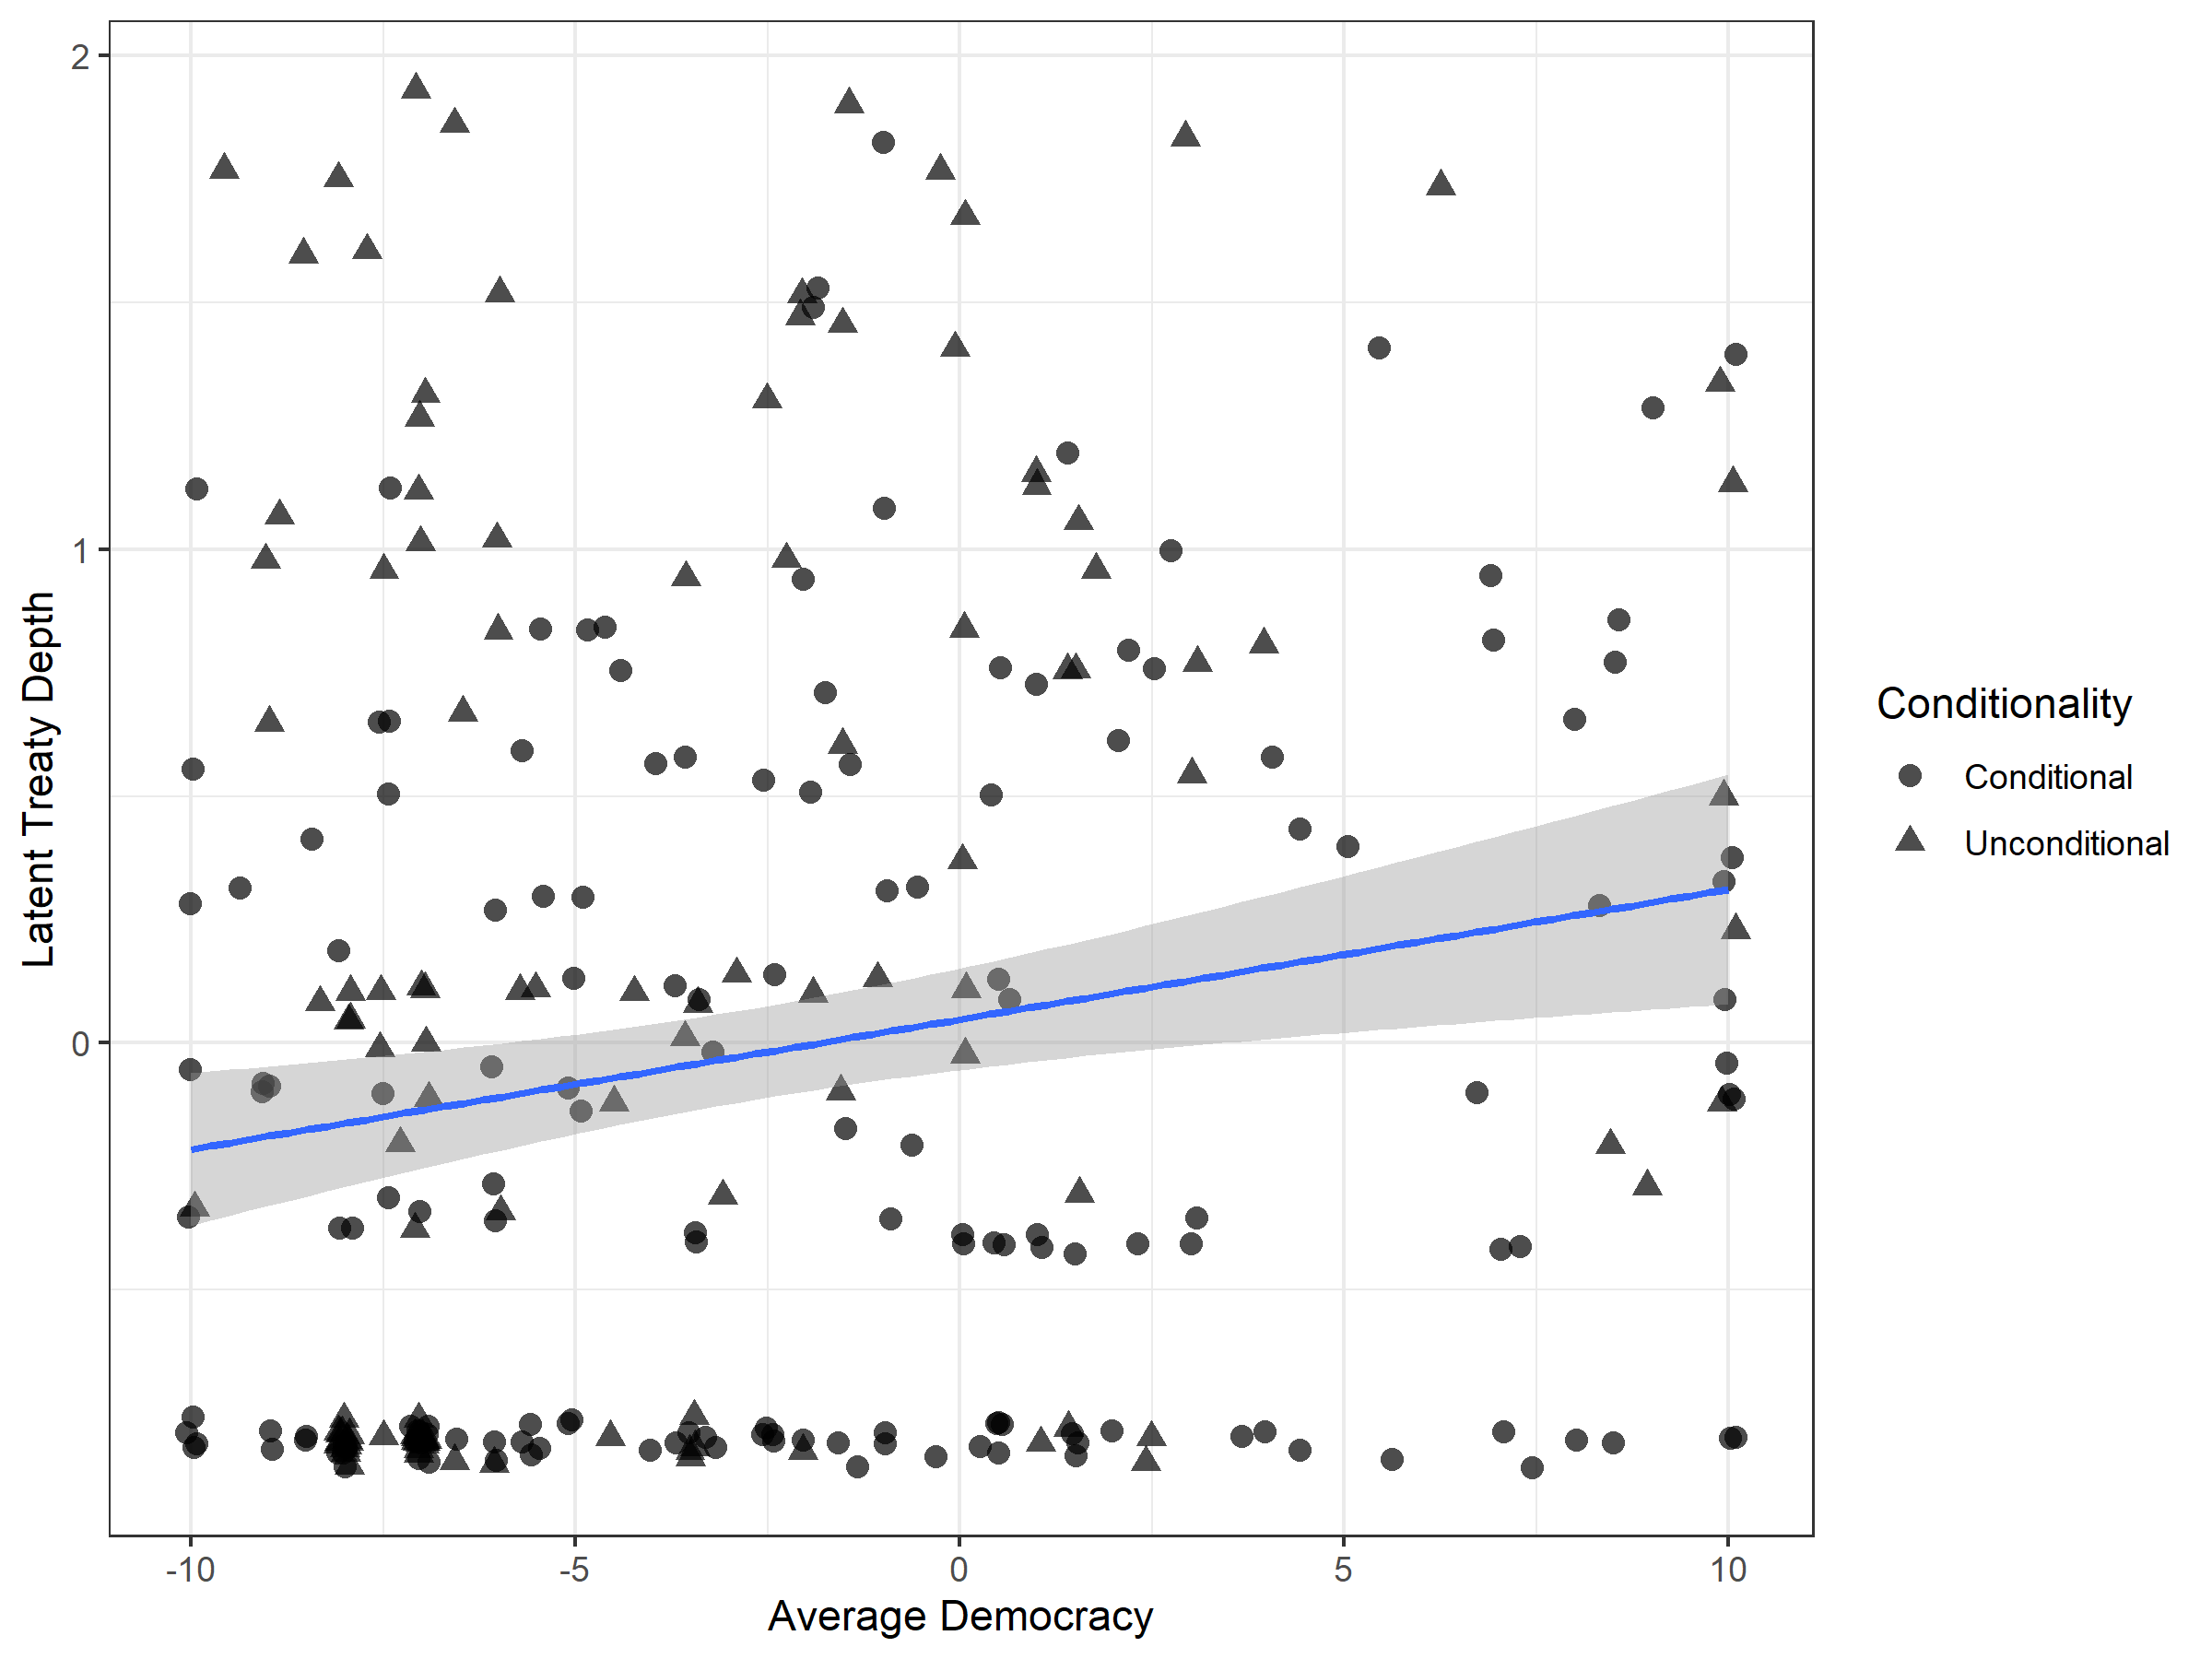
\includegraphics[width=0.95\textwidth]{../figures/democ-combo.png}
\caption{Average of the most capable alliance member's polity score when the alliance formed in four groups of alliance from 1816 to 2016. Divisions between alliances based on unconditional military support and treaty depth. Darker quadrants mark a higher average democracy score for that group of alliances, and the text in each box gives the precise value.}
\label{fig:democ-combo}
\end{figure}


These descriptive results do not adjust for potential confounding factors, however.
Therefore, I describe results from statistical models of depth and unconditional military support, starting with separate models. 
\autoref{tab:separate-models} shows results from a beta model of treaty depth and a binomial model of unconditional military support with a probit link function. 
The results are partially consistent with the hypotheses.
First, I find a positive association between the democracy of the most capable alliance member and treaty depth. 
For unconditional military support, the parameter estimate is negative, but the 95\% confidence interval for alliance leader democracy includes zero and positive values. 


\begin{table}[!htbp] \centering 
  \caption{Independent Models of Alliance Treaty Depth and Unconditional Military Support in ATOP Offensive and Defensive Alliances from 1816 to 2007.} 
  \label{tab:separate-models} 
\begin{tabular}{@{\extracolsep{5pt}}lcc} 
\\[-1.8ex]\hline 
\hline \\[-1.8ex] 
 & \multicolumn{2}{c}{\textit{Dependent variable:}} \\ 
\cline{2-3} 
\\[-1.8ex] & Latent Depth (rescaled) & Unconditional Military Support \\ 
\\[-1.8ex] & \textit{beta} & \textit{probit} \\ 
\\[-1.8ex] & (1) & (2)\\ 
\hline \\[-1.8ex] 
  Most Capable Member POLITY & 0.023$^{}$ & $-$0.018 \\ 
  & (0.002, 0.043) & ($-$0.047, 0.011) \\ 
  Foreign Policy Concessions & $-$0.057 & 0.021 \\ 
  & ($-$0.209, 0.096) & ($-$0.197, 0.239) \\ 
  Number of Members & 0.016 & $-$0.030 \\ 
  & ($-$0.011, 0.043) & ($-$0.077, 0.018) \\ 
  Wartime Alliance & $-$0.309$^{}$ & $-$0.954$^{}$ \\ 
  & ($-$0.658, 0.040) & ($-$1.570, $-$0.338) \\ 
  Asymmetric Obligations & 0.189 & 0.035 \\ 
  & ($-$0.155, 0.532) & ($-$0.467, 0.537) \\ 
  Asymmetric Capability & 0.347 & 0.651 \\ 
  & ($-$0.120, 0.814) & ($-$0.218, 1.520) \\ 
  Non-Major Only & 0.275 & 1.146$^{}$ \\ 
  & ($-$0.228, 0.779) & (0.266, 2.027) \\ 
  Average Threat & 1.248$^{}$ & 1.630$^{}$ \\ 
  & (0.376, 2.120) & (0.295, 2.965) \\ 
  Foreign Policy Disagreement & 0.197 & 0.394 \\ 
  & ($-$0.258, 0.653) & ($-$0.306, 1.094) \\ 
  Start Year & 0.004$^{}$ & 0.015$^{}$ \\ 
  & (0.0004, 0.007) & (0.010, 0.021) \\ 
  Constant & $-$8.929$^{}$ & $-$31.655$^{}$ \\ 
  & ($-$15.679, $-$2.179) & ($-$43.220, $-$20.091) \\ 
 \hline \\[-1.8ex] 
Observations & 277 & 277 \\ 
Log Likelihood & 54.349 & $-$132.467 \\ 
\hline 
\hline \\[-1.8ex] 
\textit{Note:}  & \multicolumn{2}{r}{95\% Confidence Intervals in Parentheses.} \\ 
\end{tabular} 
\end{table} 


Based on the coefficient estimates in \autoref{tab:separate-models}, I assess the substantive impact of allied democracy in \autoref{fig:results-democ-max}.
This figure plots the estimated marginal effect of the alliance leader's polity score on both outcomes. 
The left-hand plot of \autoref{fig:results-democ-max} shows the association between the democracy of the most capable alliance member and the predicted probability of unconditional military support. 
This relationship is weaker than expected.  
These results diverge from previous findings that democratic alliance membership leads to limited obligations \citep{Mattes2012, Chibaetal2015}.


\begin{figure}[hbtp]
\centering
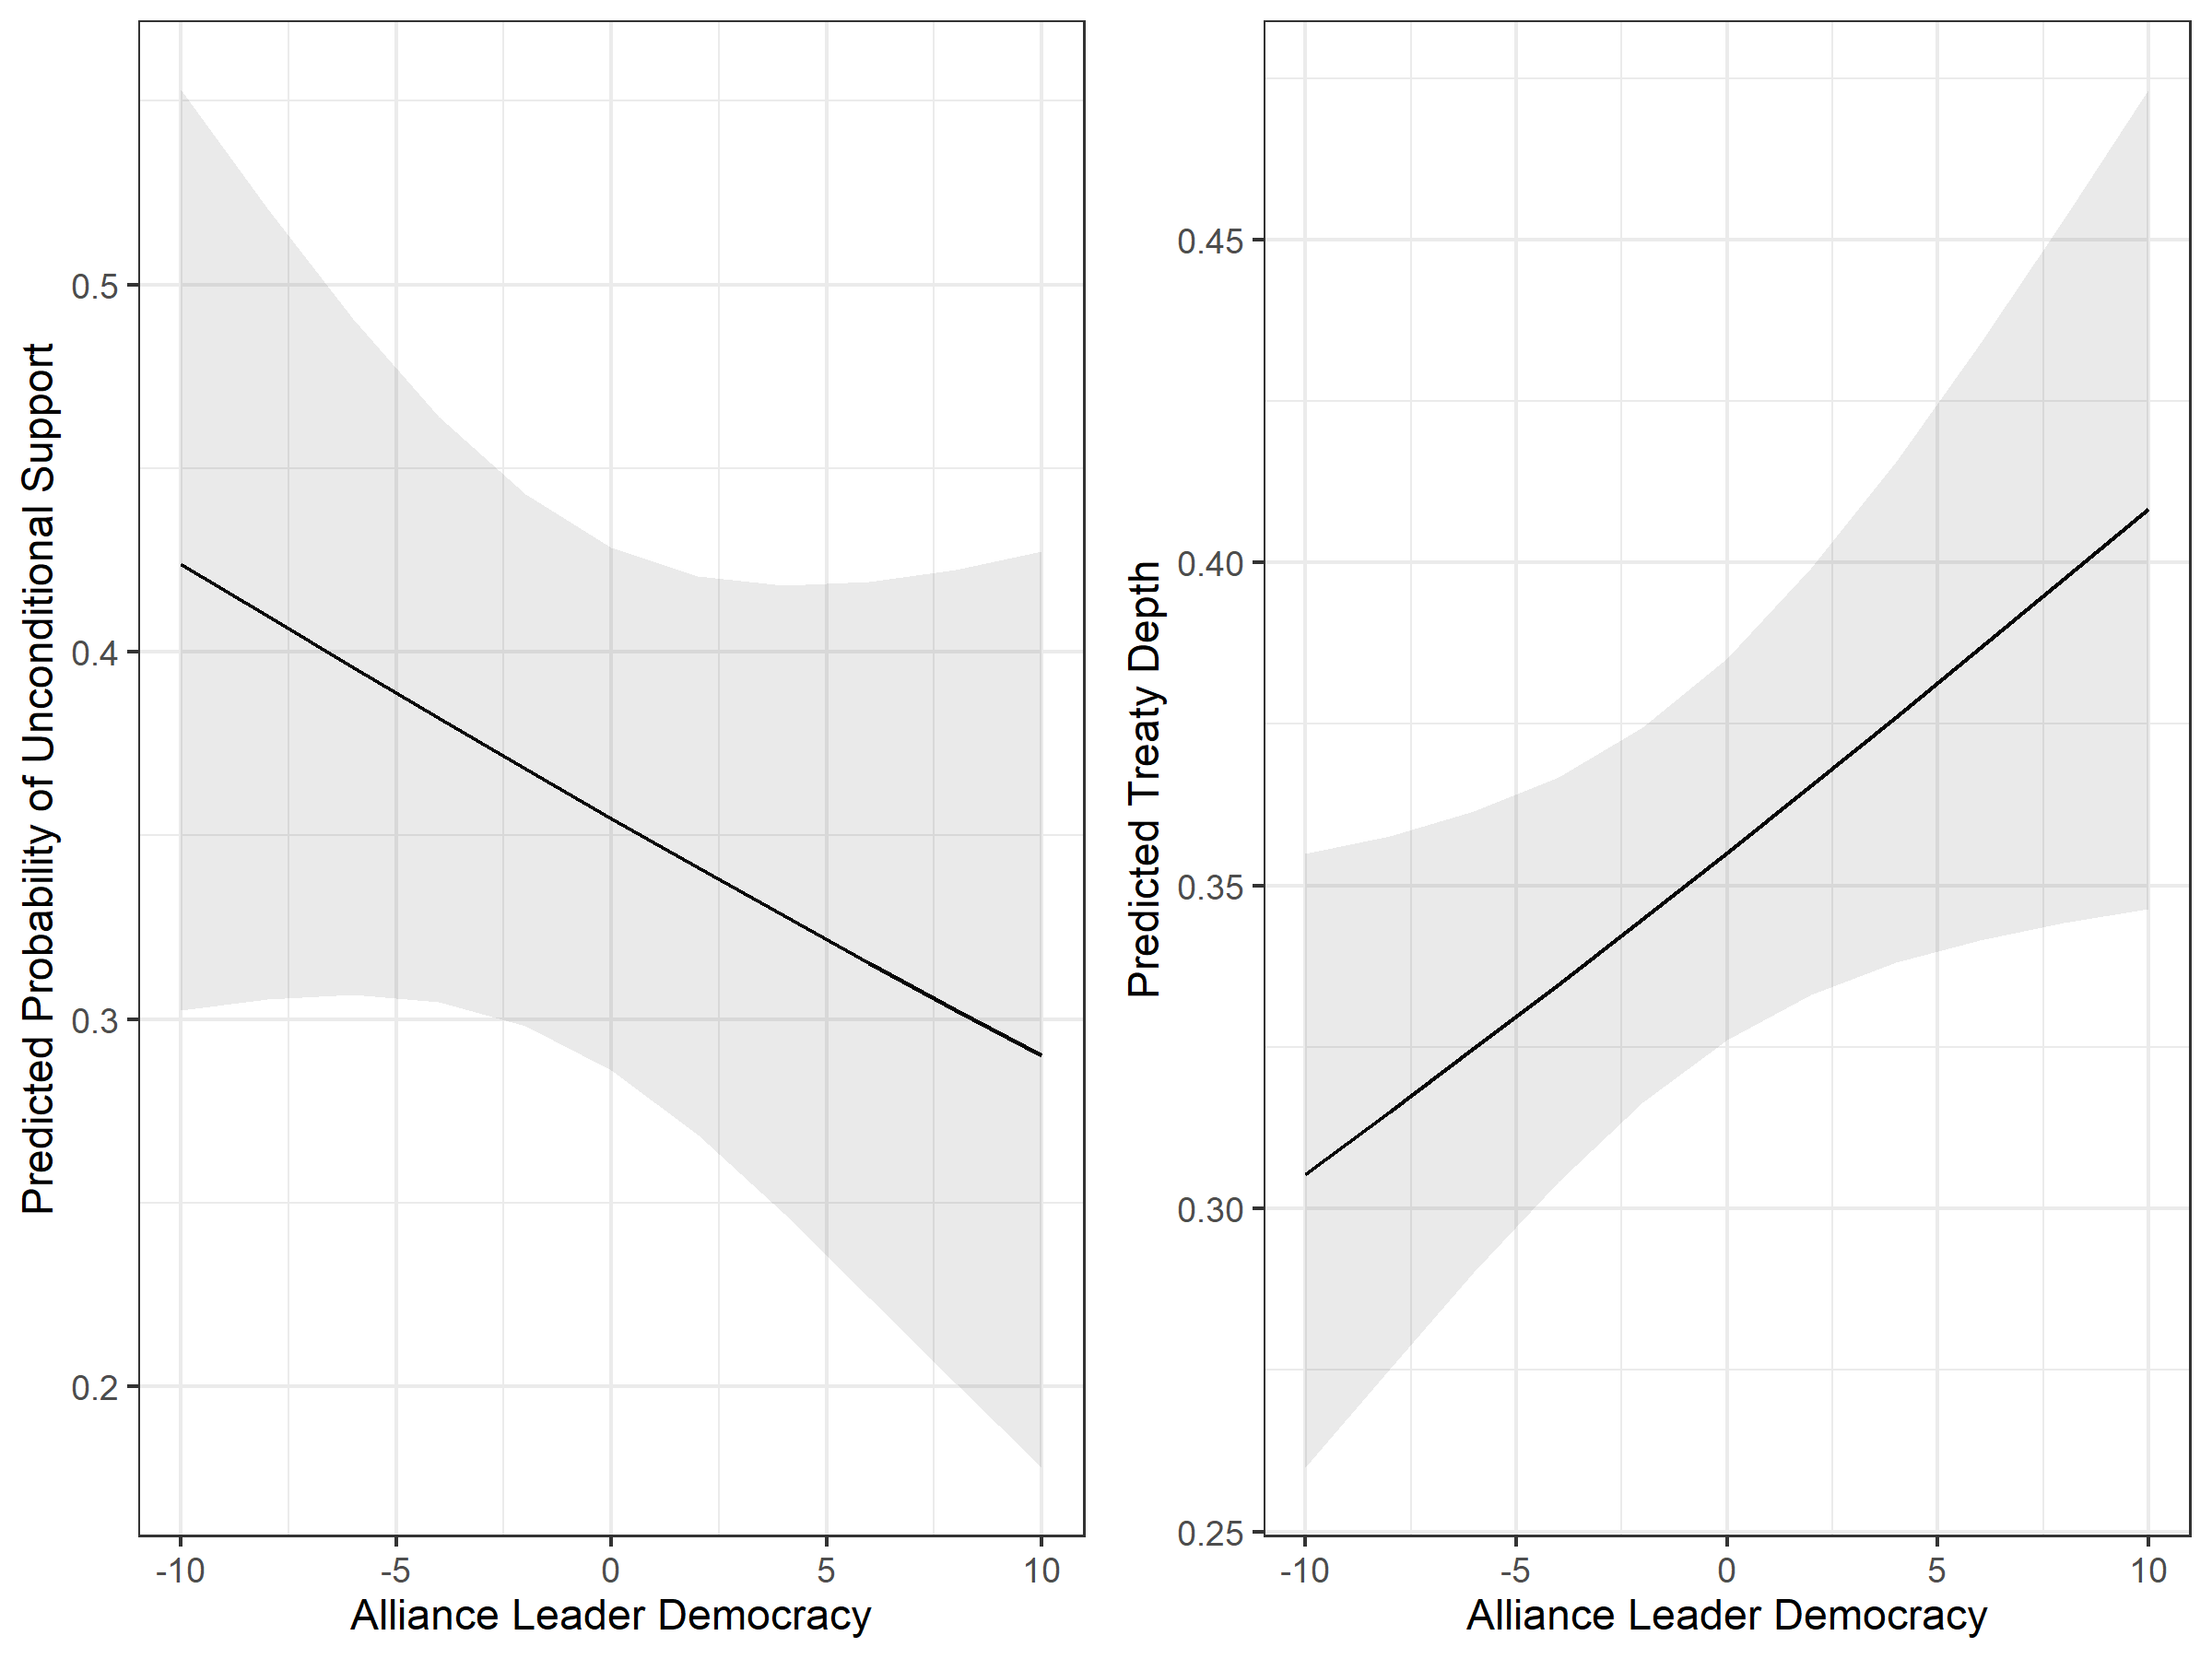
\includegraphics[width=0.95\textwidth]{../figures/results-democ-max.png}
\caption{Predicted probabilities of unconditional military support and predicted change in treaty depth across the range of average alliance democracy. The line marks predicted values, and the shaded areas encapsulate the standard errors. The rug plot on the x-axis marks observed values of allied democracy. Predictions based on the smoothed terms from a joint generalized regression model.}
\label{fig:results-democ-max}
\end{figure}


The right-hand plot in \autoref{fig:results-democ-max} shows a positive relationship between average democracy at the time of alliance formation and treaty depth.
A highly democratic alliance leader leads to greater treaty depth. 
The predicted value of rescaled treaty depth in an alliance with a fully democratic leader is roughly .1 greater than an alliance with a fully autocratic leader, in expectation. 
This substantively large relationship matches the treaty depth hypothesis.


Although the results from separate models are informative, they do not account for correlations in the error terms of the depth and unconditional support models, which could affect inferences. 
I now report the results of a bivariate model of depth and unconditional military support in \autoref{tab:gjrm-res}. 
This table contains results from both equations of the GJRM model, and marks smoothed terms with the letter s. 


As in \autoref{tab:separate-models}, I find a positive relationship between the democracy of the leading alliance member and treaty depth, but a weak negative relationship between democratic influence and treaty depth.  
The control variables in this model are also interesting and somewhat different from the estimates in the separate models.  
Asymmetric capability in an alliance and symmetric alliances between non-major powers are more likely to include unconditional military support than symmetric major power alliances. 
I also find that the number of members and wartime alliances reduce the probability of unconditional military support. 
Asymmetric capability and the number of alliance members both increase depth. 
Last, threat and the year of alliance formation increase unconditional military support and treaty depth. 


\begin{table}[ht]
\centering
\begin{tabular}{lrrrr}
  & \multicolumn{2}{c}{Uncond. Mil. Support} & \multicolumn{2}{c}{Latent Depth}\\ \hline
  & Estimate & Std. Error & Estimate & Std. Error \\ 
  \hline
  Most Capable POLITY & -0.0173979 & 0.0158094 & 0.0262429 & 0.0097732 \\ 
  Economic Issue Linkage & 0.2232389 & 0.2006227 & -0.0060972 & 0.1458203 \\ 
  FP Concessions & -0.1468542 & 0.1214414 & -0.0339923 & 0.0845875 \\ 
  Number of Members & -0.0994788 & 0.0264666 & 0.0179032 & 0.0129499 \\ 
  Wartime Alliances & -0.6274650 & 0.3157751 & -0.0744869 & 0.1787959 \\ 
  Asymmetric Obligations & -0.0181268 & 0.2622665 & 0.1686232 & 0.1632100 \\ 
  Asymmetric Capability & 0.9586816 & 0.3864164 & 0.3436770 & 0.2192153 \\ 
  Non-Major Only & 1.7040882 & 0.3975041 & 0.0828621 & 0.2310327 \\ 
  FP Disagreement & 0.1253382 & 0.3352438 & 0.3284441 & 0.2204690 \\ 
  s(Mean Threat) & 7.3253441 & 43.4564525 & 1.0000004 & 16.8780421 \\ 
  s(Start Year) & 4.7057429 & 49.8605879 & 3.3275472 & 39.7155651 \\
  (Intercept) & -1.0980618 & 0.4635789 & -1.0810691 & 0.2485382 \\  
   \hline
\end{tabular}
\caption{Results from joint generalized regression model of treaty depth and unconditional military support. 
                     All smoothed terms report the effective degrees of freedom and the chi-squared term. 
                     The unconditional military support model is a binomial GLM with a probit link function. 
                     The treaty depth model is a beta regression. 
                     I model the error correlation between the two processes with a T copula.} 
\label{tab:gjrm-res}
\end{table} 


I make similar inferences about democracy and treaty design with univariate and bivariate models.
Inferences about the control variables vary somewhat across the two models, so accounting for correlated errors is worthwhile.   
I find that the polity score of the most capable alliance member is positively correlated with treaty depth, and has a slight negative association with unconditional military support.


\subsection{Elections, Political Competition and Executive Constraints} 


Having analyzed cumulative democracy scores, I now turn to a model that distinguishes between the different parts of the POLITY index. 
The key independent variables in this model are dummy indicators of competitive elections, open political competition, and executive constraint through parity or subordination to other actors. 
All three of these factors could contribute to audience costs by exposing leaders to adverse reactions to foreign policy actions. 
I use a bivariate GJRM model to assess this relationship.\footnote{A T copula has the best model fit and AIC.} 


\begin{table}[ht]
\centering
\begin{tabular}{lrrrr}
 & \multicolumn{2}{c}{Uncond. Mil. Support} & \multicolumn{2}{c}{Latent Depth}\\ \hline
   & Estimate & Std. Error & Estimate & Std. Error \\ 
  \hline 
  Competitive Elections & -1.3862036 & 0.5969913 & 1.0334447 & 0.3441959 \\ 
  Political Competition & 0.1267747 & 0.4456283 & -0.3968825 & 0.2894709 \\ 
  Executive Constraints & 0.7810824 & 0.2758115 & -0.3806161 & 0.2006471 \\ 
  Economic Issue Linkage & 0.0786646 & 0.1830420 & 0.1099506 & 0.1466334 \\ 
  FP Concessions & -0.1284395 & 0.1256934 & -0.1052689 & 0.0817796 \\ 
  Number of Members & -0.1004983 & 0.0271633 & 0.0268154 & 0.0139085 \\ 
  Wartime Alliances & -0.7495699 & 0.2448796 & 0.0599420 & 0.1700357 \\ 
  Asymmetric Obligations & -0.0230173 & 0.2251492 & 0.1766837 & 0.1620580 \\ 
  Asymmetric Capability & 1.0281801 & 0.5255088 & 0.4985258 & 0.2426731 \\ 
  Non-Major Only & 1.6291469 & 0.5180102 & 0.1175974 & 0.2551236 \\ 
  FP Disagreement & 0.1726706 & 0.2975962 & 0.3405041 & 0.2124881 \\ 
  s(Mean Threat) & 7.5870610 & 44.8092434 & 1.0000005 & 25.8169433 \\ 
  s(Start Year) & 5.9742148 & 50.0279652 & 8.3362695 & 57.7689902 \\ 
  (Intercept) & -0.8925660 & 0.6081549 & -1.3310577 & 0.2833844 \\
   \hline
\end{tabular}
\caption{Results from joint generalized regression model of treaty depth and unconditional military support as a function of competitive elections, political competition and executive constraints. 
                     All smoothed terms report the effective degrees of freedom and the chi-squared term. 
                     The unconditional military support model is a binomial GLM with a probit link function. 
                     The treaty depth model is a beta regression. 
                     I model the error correlation between the two processes with a T copula.} 
\label{tab:gjrm-res-split}
\end{table}


The three components of democracy have different consequences for alliance treaty design.
First, the presence of competitive elections decreases the probability of unconditional military support and increases treaty depth.
This matches the argument--- if leaders can be removed from office by competitive elections, they prefer treaty depth to unconditional military support because depth is less salient for voters. 
Second, the political competition coefficient for treaty depth is negative, albeit with substantial uncertainty. 
This implies that scrutiny of the executive from open political competition may restrain deep alliance commitments. 
Political competition has little association with the probability of unconditional military support. 


Last, executive constraints has the opposite effect of electoral competition on both credibility sources, which is interesting and unexpected.
First, I find that executive constraints reduce treaty depth.  
Constraints might reduce treaty depth by exposing the executive to scrutiny from other political elites who have ample information about foreign policy and want to avoid foreign entanglements.  
Second, domestic institutions with executive parity or subordination increase the probability of unconditional military support.  
One explanation for the positive relationship between constraints and unconditional support is that democratic leaders want to commit successors with different foreign policy preferences to the alliance \cite{Mattes2012a}. 
Leadership turnover in democracies threatens international cooperation, because new leaders may have different supporters and preferences \citep{Lobell2004, Narizny2007, Leedsetal2009}. 
By making an unconditional promise of military support, leaders generate higher audience costs for successor governments to break the alliance. 


Taken together, the results from dividing democratic institutions help explain the results from the aggregate democracy measure. 
A large positive effect of competitive elections drives the positive association between democracy and treaty depth, as it overwhelms the smaller negative effect of executive constraints. 
Competitive elections decrease the probability of unconditional military support, but executive constraints make unconditional support an attractive way to precommit future leaders to the alliance. 
Because these competing effects cancel each other out, there is a weak association between the democracy of the alliance leader and the probability of unconditional military support. 


These statistical results give mixed evidence for the argument. 
Democracies do form deeper treaties, but democratic institutions have competing effects on the probability of unconditional military support. 
To further examine my claim that democracies often use treaty depth to reassure, but are less inclined to offer unconditional support, I describe how US preferences shaped the institutional design of NATO. 


\subsection{NATO Treaty Design}


I focus this brief case study on NATO treaty design for two reasons. 
First, the process behind NATO applies to multiple alliances, as other US treaties have similar designs. 
Second, NATO is also the most important alliance in international politics, so understanding how the treaty formed is worthwhile. 


After the end of World War II, the US sought a way to protect Europe from the USSR. 
Despite acute security concerns, fear of entrapment in unwanted conflicts led to limits on military support. 
First, as \citet{Poast2019a} details, NATO members disagreed over how to define the North Atlantic area, which was a key condition on military support. 
The US and other states argued about whether France's Algerian colony and Italy should be protected by the alliance. 
Second, active military support from NATO members depends on domestic political processes.\footnote{\citet{Benson2012} calls this kind of commitment a ``probablistic'' obligation.} 
Isolationists in the US Senate feared that an alliance would force America to intervene automatically if partners were attacked, bypassing the power of Congress to declare war and engaging the US in unwanted conflicts \citep[pg. 280-1]{Acheson1969}.
Therefore Article V of the NATO treaty states that if one member is attacked the others ``will assist the Party or Parties so attacked by taking forthwith, individually and in concert with the other Parties, \emph{such action as it deems necessary} (emphasis mine).'' 
Military support was and is not guaranteed. 
Secretary of State Dean Acheson stated as much in a March 1949 press release defending NATO to the US public, where he said that Article V ``does not mean that the United States would automatically be at war if one of the nations covered by the Pact is subject to armed attack'' \citep{Acheson1949}.
This claim and the emphases of the press release shows that promises of military support were highly salient to the US public.


Military support from Article V did not assuage European fears that if the Soviets invaded, the United States would not fight. 
To increase the credibility of NATO, the United States took other measures.  
A 1951 presentation by Dean Acheson to Dwight Eisenhower argued European allies ``fear the inconstancy of United States purpose in Europe. ... These European fears and apprehensions can only be overcome if we move forward with determination and if we make the necessary full and active contribution in terms of both military forces and economic aid'' \citep[pg. 3]{Acheson1951}. 


The first part of reassurance was the creation of the Atlantic Council, which is an international organization and the main source of depth in the NATO treaty itself. 
The United States used the Atlantic Council to coordinate collective defense and increase the perceived reliability of the alliance. 
By investing in the Atlantic Council and related joint military planning, the US addressed European fears of abandonment. 
For example, US officials thought that the British Foreign Minister viewed US provision of a supreme commander in Europe as ``a stimulus to European action'' in NATO \citep{Acheson1950}. 


Many Senators also opposed military aid to Europe \citep[pg 285]{Acheson1969}, which limited efforts to add further treaty depth. 
Thus, legislative constraints on the executive branch reduced the formal depth of NATO relative to what many ambassadors preferred \citep[pg 277]{Acheson1969}. 
Bilateral agreements on troop deployments then became another instrument of reassurance. 
In 1950 the Germans formally requested clarification on whether an attack on US forces in Germany would be treated as an armed attack on the US- which the US said it would \citep[pg. 395]{Acheson1969}.  
These bilateral arrangements and basing rights are not covered in the NATO treaty, but they added substantial depth.\footnote{This is a potential limitation of the statistical models.}  


% Sum up 
NATO negotiations reveal the tendency of democracies to use treaty depth to reassure their allies, rather than unconditional military support. 
Fear of foreign entanglement led the United States to offer conditional military support, but did not inhibit deep military cooperation, which helped reassure European allies. 
Limits on the promises of military support were an important public justification for the NATO treaty, while the Atlantic Council was less discussed. 
Still, the power of treaty ratification in the Senate limited formal NATO depth to the Atlantic Council. 
The Atlantic Council and associated bureaucratic machinery are the formal core of substantial defense cooperation. 
Altogether though Article V is limited, the US used treaty depth to increase the credibility of NATO. 



\section{Discussion and Conclusion}


% main evidence for an indirect effect
The findings from the statistical models and case study of NATO generate mixed evidence for the hypotheses. 
I find regular evidence that democracies often form deep alliances, which may be driven by selecting leaders through open elections.  
There is inconsistent support for claims that allied democracy decreases the probability of unconditional military support, however, because competitive elections and executive constraints have contradictory effects. 
Elections encourage conditional obligations, but executive constraints may encourage locking successors into the alliance with unconditional support. 


% this evidence suggests
The results are mostly consistent with my overarching claim states form deep alliances to increase the credibility of their alliance commitments while managing the risk of entrapment and audience costs. 
Because democracies are concerned with audience costs and treaty depth has little salience with voters, they often use treaty depth to increase the credibility of their alliances.
Electoral politics are largely responsible for this relationship, and they also push democracies away from unconditional military support. 


% limitations
My argument and evidence have two limitations. 
For one, I only examine variation in formal treaty design. 
This omits the implementation of alliance promises, which may be deeper or shallower than the treaty language alone implies. 
As the NATO case study shows, formal treaty depth reflects practical depth, but it may miss some differences between alliances. 
Changes in realized alliance depth are a useful subject for future inquiry, but will require new data collection.
Also, the small sample size of observed alliances adds uncertainty to inferences.  


Despite its limitations, this paper has four main implications for scholarship. 
First, one reason treaty depth matters is that it affects military spending by alliance participants.
The findings in this paper imply that states do not use treaty depth to manipulate allied military spending, but rather to increase the credibility of the alliance. 
Therefore, treaty depth is non-randomly selected based on observable alliance characteristics like domestic institutions, but selection on unobservable preferences over allied military spending is less likely. 


Second, studies of how alliance participation affects international politics must account for alliance design and membership. 
Alliance member characteristics and treaty design are correlated, and both affect the consequences of treaty participation.   
Estimating the impact of member characteristics alone, or treaty design alone, risks omitted variable bias. 


The third implication is that democracies do not make limited alliance commitments. 
Even if democracies impose conditions on military support, deep alliances add substantial foreign entanglement.
The most limited alliances possible would have conditional obligations and no depth.  
Last, some of the lessons from this work add to the extensive literature on the design on international institutions \citep{DownesRocke1995, MartinSimmons1998, Koremenosetal2001, Koremenos2005, Thompson2010}.
Just as democracies use depth to support allies while managing electoral risks, democracies may undertake international commitments in ways that limit public scrutiny. 


The findings also raise at least two questions for future research.  
First, they address debates about whether democracies make more credible commitments than other states. 
The effect of democracy on credibility can be divided into conditions on military support, treaty depth, and the direct effect of institutions and domestic politics. 
These may have competing or conditional effects, which could explain mixed findings about the credibility of democratic commitments \citep{Schultz1999, Leeds1999, Thyne2012, DownesSechser2012, PotterBaum2014}.
Future research should combine the components of democracy and democratic alliances to asses the net effect of democracy on credible commitment in international relations. 


Scholars should also consider how alliance treaty design varies among different types of autocracies. 
As I noted in the argument, some autocratic states have high audience costs for backing down in military interventions. 
Differences in the salience of audience costs, which actors impose audience costs on leaders and what information those actors have about foreign policy \citep{Weeks2008} may help explain alliance treaty design.
For example, personalist leaders with few public or elite constraints on their foreign policy may be able to form alliances with depth and unconditional military support. 


In conclusion, states use deep alliances to reassure their partners while limiting the risk of entrapment. 
Domestic political institutions shape how states build the credibility of their alliances.
Thanks to high audience costs of military intervention, democracies are especially likely to use treaty depth to increase the credibility of their alliances. 



\singlespace
 
\bibliography{../../../MasterBibliography} 





\end{document}
